\clearpage
\appendix
\section{Additional figures}
\begin{figure}[ht]
  \centering
  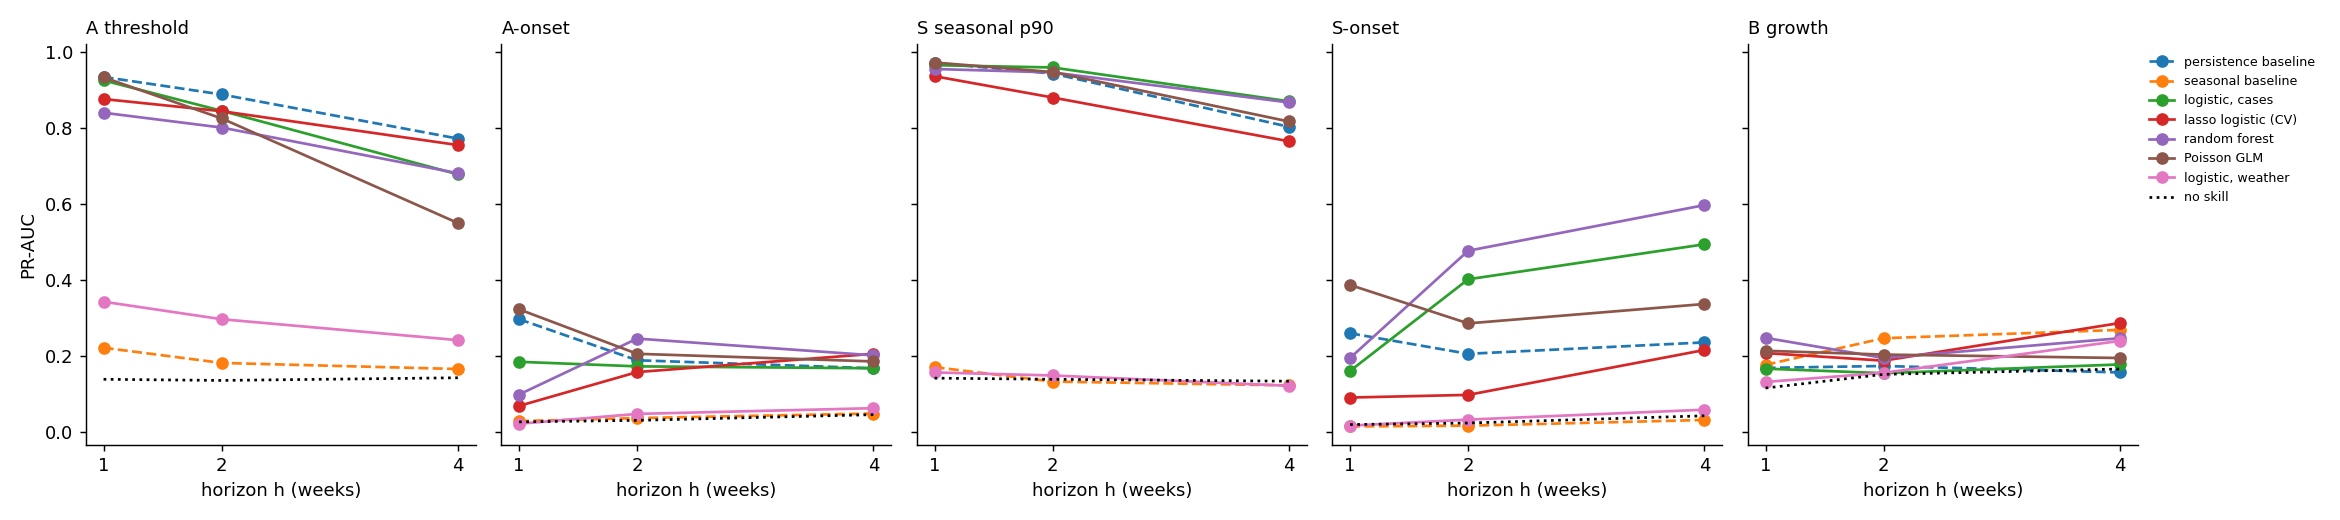
\includegraphics[width=\linewidth]{04_pr_auc_by_horizon.png}
  \caption{Development PR-AUC by horizon for each surge definition.}
\end{figure}
\begin{figure}[ht]
  \centering
  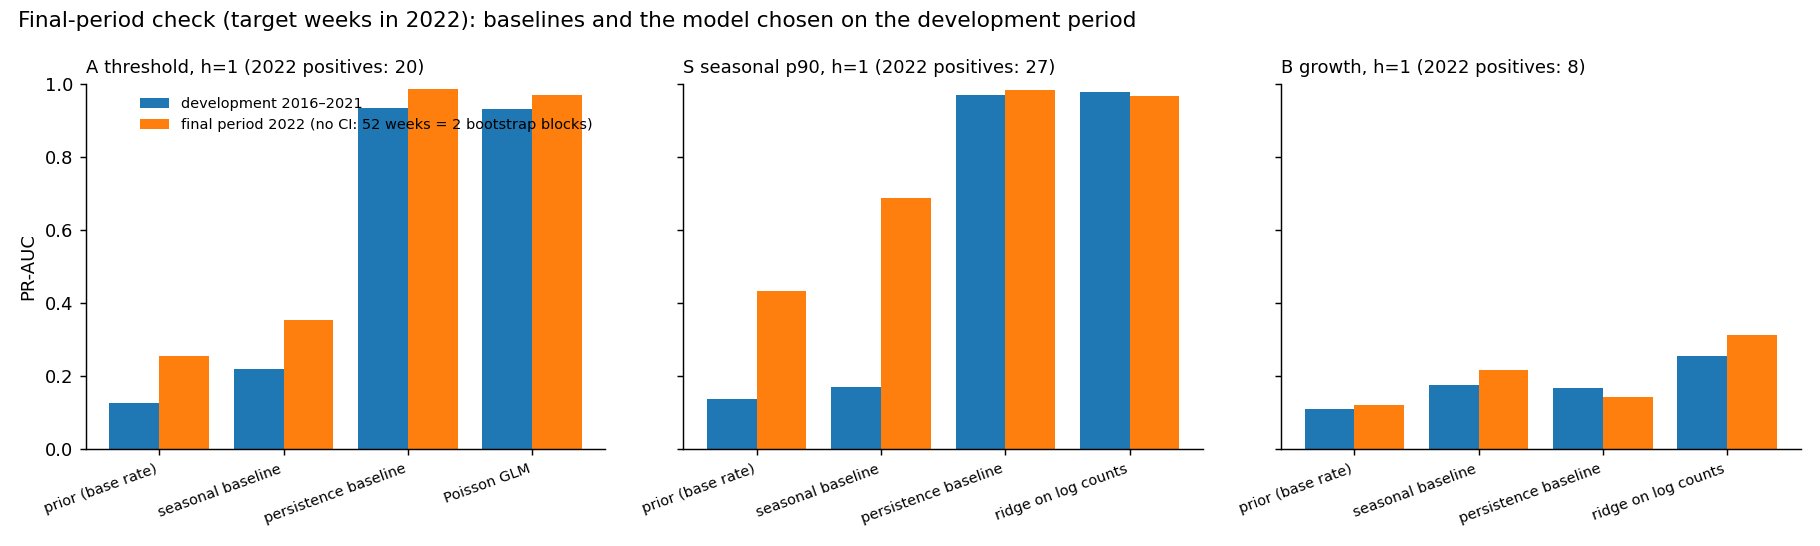
\includegraphics[width=\linewidth]{12_final_test_holdout_h1.png}
  \caption{Development vs.\ 2022 PR-AUC for the baselines and the development-selected model, $h=1$.}
\end{figure}
\begin{figure}[ht]
  \centering
  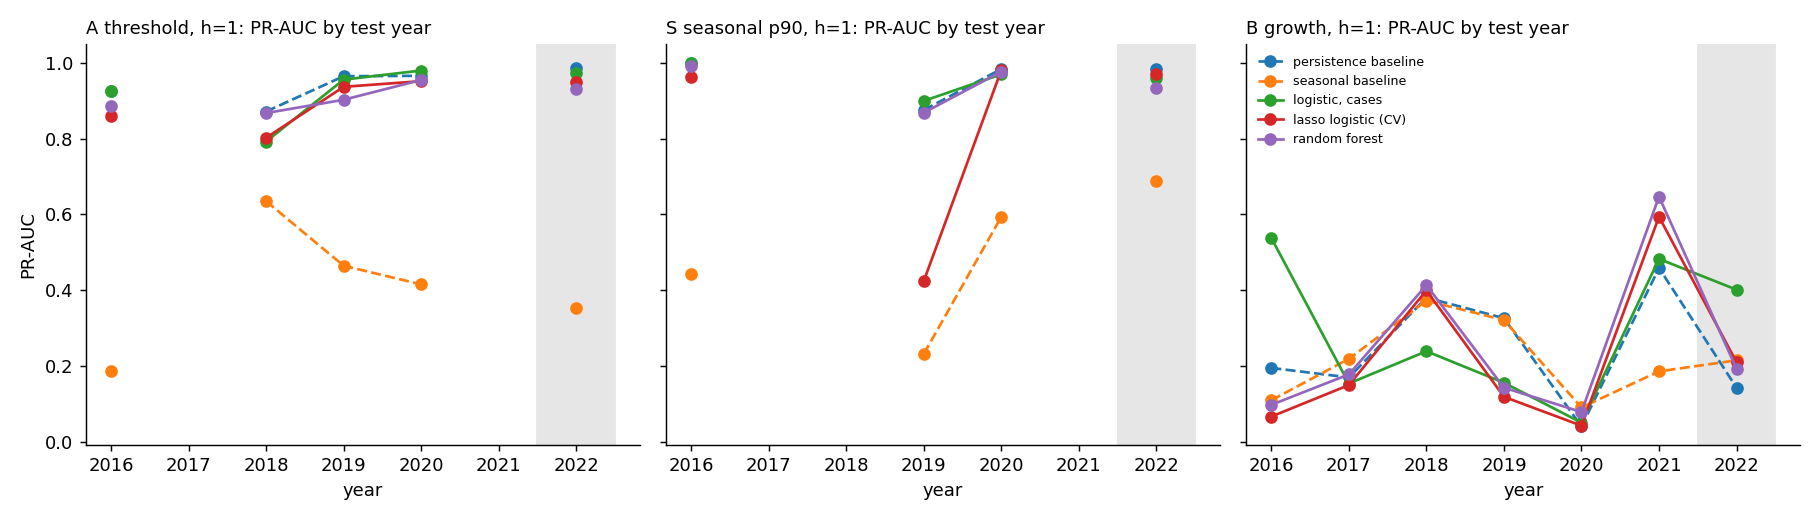
\includegraphics[width=\linewidth]{07_pr_auc_by_year_h1.png}
  \caption{PR-AUC by target year, $h=1$; 2022 is the final period.}
  \label{fig:byyear}
\end{figure}
\begin{figure}[ht]
  \centering
  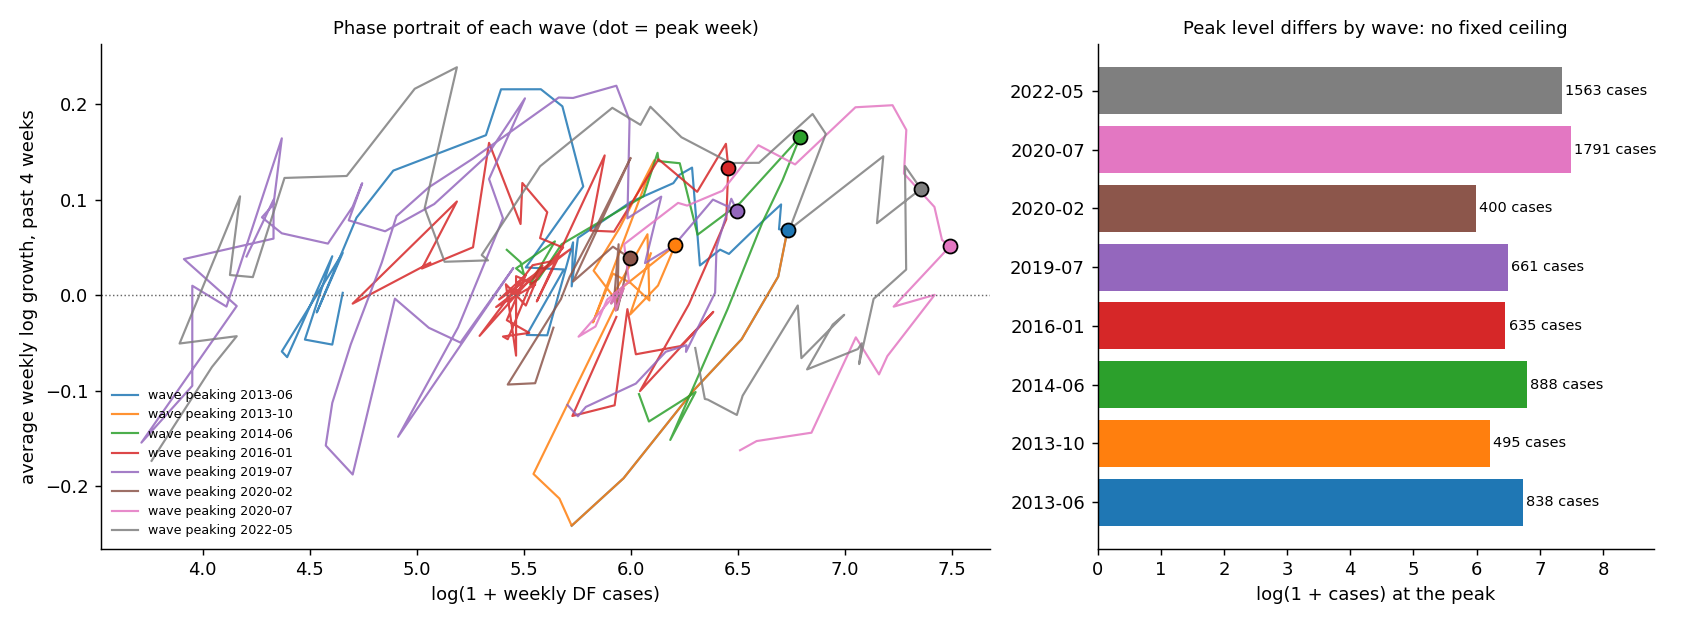
\includegraphics[width=\linewidth]{peak_01_phase_portrait.png}
  \caption{Exploratory: growth against level for each wave (dot = peak week) and the level at
  each peak. Peaks occur at different levels and often while growth is still positive.}
  \label{fig:phase}
\end{figure}
\begin{figure}[ht]
  \centering
  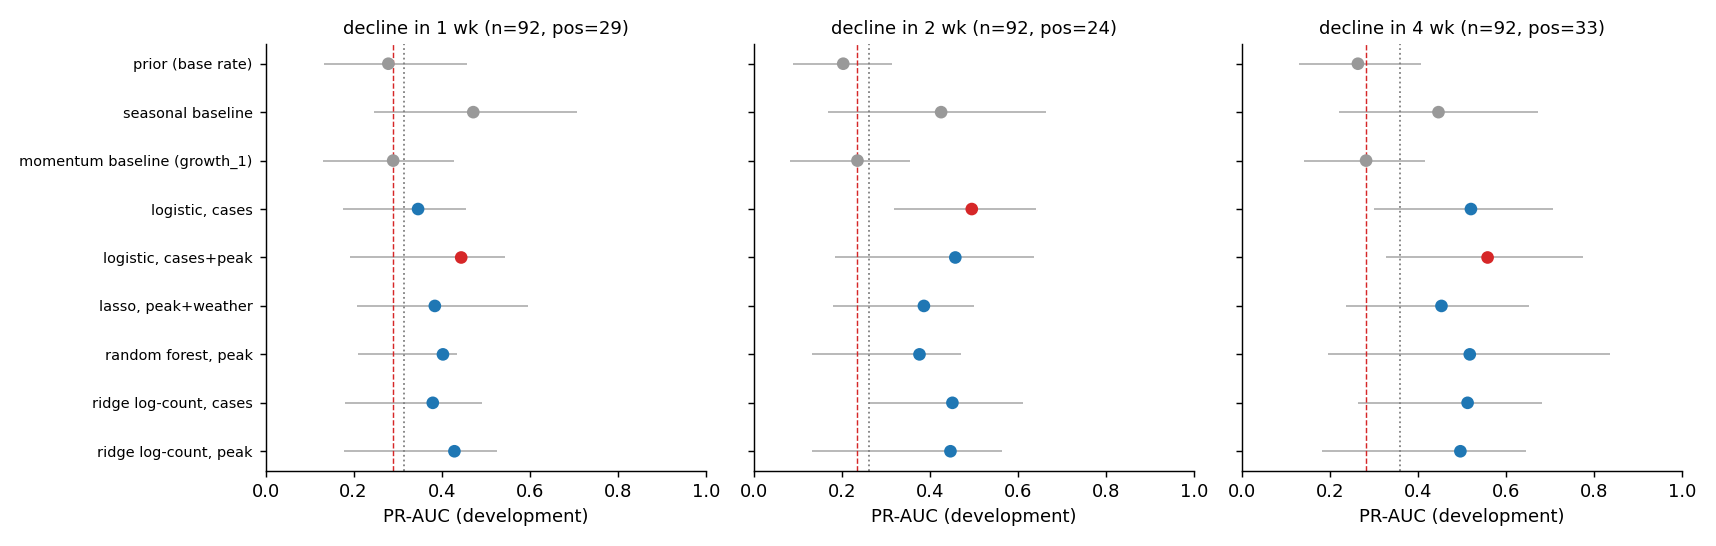
\includegraphics[width=\linewidth]{peak_03_pr_auc.png}
  \caption{Exploratory decline targets: development PR-AUC with 95\% block-bootstrap intervals
  (13-week blocks). Dotted: base rate; red dashed: momentum baseline; red dot: best model.}
  \label{fig:peakprauc}
\end{figure}
\begin{figure}[ht]
  \centering
  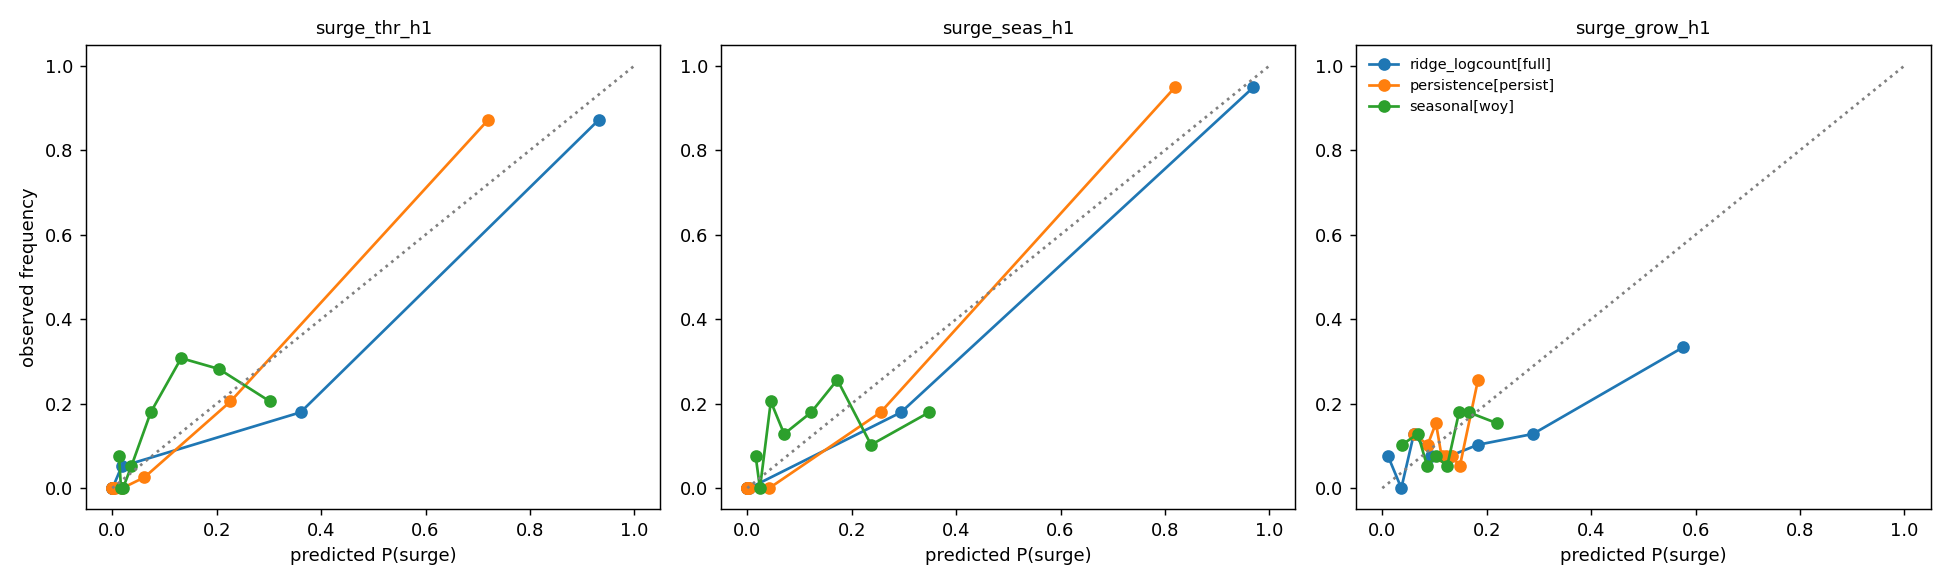
\includegraphics[width=0.75\linewidth]{05_calibration_h1.png}
  \caption{Calibration (development period, $h=1$) of the best model, persistence and the seasonal baseline.}
\end{figure}
